\chapter{Versioning}
\label{chap:versioning}

Versioning determines creation and management of product versions. The product is what a provider offers to a consumer. Consumers can use the same product but they can use its different version. A version of a product can be created when a modification is needed or due to improvements of functionality.

In service oriented architecture the services as they are described in section \ref{sec:services} are the product. Provider is the one who provide services - server. Consumer is the one who use services - client.

Any changes of the product mustn't influence the execution of consumers code.
When the product is customized, a change has to be compatible with all consumers. In case the change is incompatible, it is needed to produce a new version. Types of changes are described in next section.


\section{Version compatibility}
\label{sec:v-compat}
The changes which can be done within the services can have different impact on consumers. One type does not require changes on client side the other one on the contrary does. There are two forms of compatibility between the service versions. \cite{website:service-versioning}

\subsection{Compatible changes}
  Compatible changes are changes of a product which do not affect existing consumer functionality. Compatible changes are for example implementation bug fixes or additions of parameters in interface to support an implementation modification.
  \begin{enumerate}
    \item[Backward compatible] \hfill \\ 
  When a new version of a service is deployed the consumer of an earlier version must be able to interoperate with the new version without any modification of his application. If a service update, is backward compatible it is compatible with older version of itself. Backward compatible change can be an addition of a new resource or a new capability to the resource. \hfill \\ 
  Example: \hfill \\ 
  Service has an action which is sent with \gls{queries} \hfill \\ 
  \begin{lstlisting}
  GET   /customers?name={name}
  \end{lstlisting}
  The query is a search paramater. It returns a customer with particular name. A new query is added to the service. It allowes to find a customer with listed surname. 
  \begin{lstlisting}
  GET   /customers?name={name}&surname={surname}
  \end{lstlisting}

  The additon of an optional query parameter is a compatible change. It doesn't harm any consumers because they can continue to use every capability which has been already integrated.
  
  \item[Forward compatible] \hfill \\
  The service version is forward compatible when it is designed in a way it can support future modifications. It is hard to achieve the forward compatibility because its about unknown future changes which can be done. Services should be designed in a way that they can be modified.
  \end{enumerate}
  
\subsection{Incompatible changes}
  Incompatible are the breaking changes which affect consumers of services. Breaking changes can be performed by adding or removing an enumeration, removing or renaming a global type or element, changing the optionality of an element from optional to required.
  \begin{enumerate} 
    \item[Backward incompatible changes]  \hfill \\
    Backward incompatible changes are changes which break the consumers using an earlier version of service. It means that the new version is no longer compatible with earlier version of itself. It can't interpret the data of its earlier version or interprets them in wrong manner.
    
    As an example there is a service \emph{Customers}. Service has an action POST which stores a new customer. The request contains a customer representation in json format: 
    
\begin{lstlisting}
    POST   /customers
    Content-Type: application/json
    
    {
    "Name": "Peter",
    "Surname": "Sun",
    "DateOfBirth": "20 May 1978",
    "Address": {
        "Line1": "Road 23",
        "Line2": "London",
        "PostalCode": "AA0000A"
        }
    }
\end{lstlisting}

If the element \emph{DateOfBirth} is removed from the service interface it will be a breaking change. The clients would send requests containing the DateOfBirth element which wouldn't be processable. To use the new version of customers service client have to integrate the changes. 

    \item[Forward incompatible changes] \hfill \\
    These changes break the forward compatibility of the service. It means that a future version won't be compatible with existing one, any modifications of current version don't preserve compatibility.
  \end{enumerate}

\section{Versioning strategy}
\label{sec:version-strategy}
A set of rules has to be specified to version services consistently. The rules are the matter of SOA governance and form the versioning strategy. Versioning strategy defines how and when a new service version is created. It sets the approach to access the version and how many versions are accessible at the same time. Defined strategy should be followed and practiced during whole service lifecycle. 

There are three common strategies \cite{soa-governance}:

\begin{description}
  \item[Strict]  \hfill \\
  Any change of a service results in a new version as shown on the figure \ref{fig:strict-strategy}. This strategy does not support backward or forward compatibility because every modification results in a new version. This approach is the safest one and can be in place when there is a sensitive data exchange between two organizations. Consumer organization have a control over the services evolution. If any change is done the service version increases and client has to integrate it. 
    
\begin{figure}[htp] \centering{
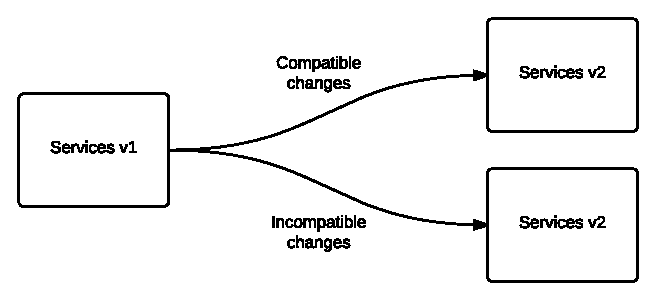
\includegraphics[width=8cm]{img/strict-strategy.pdf}}
\caption{Strict strategy versioning}
\label{fig:strict-strategy}
\end{figure} 

  \item[Flexible] \hfill \\
  Any incompatible changes results in a new version and the service design supports backward compatibility (figure \ref{fig:flexible-strategy}). This is the mostly used approach. Changes which are backward compatible modify the service interface without affecting the service version. They are considered safe and do not impact any client.
  
  \item[Loose] \hfill \\
  Any incompatible changes result in a new version and the service design supports backward and forward compatibility. The strategy is similar to Flexible one. Incompatible changes results in a new version (figure \ref{fig:flexible-strategy}). The difference is in supporting forward compatible changes. Service interface is designed in a way the future changes can be made without a breaking change.
\end{description}

\begin{figure}[htp] \centering{
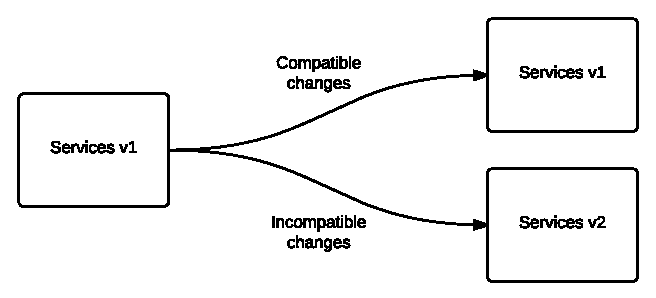
\includegraphics[width=8cm]{img/flexible-strategy.pdf}}
\caption{Flexible and Loose strategy versioning}
\label{fig:flexible-strategy}
\end{figure} 

The provider of services chooses the suitable strategy during the analysis stage of application lifecycle. It includes more decisions regarding versioning, such as version identification by digits and version lifecycle. A description of these two follows.

\subsection{Version identifiers}
\label{subsec:versionid}
Version Identification is one of the fundamental \gls{design-patterns}. Version is indicated by decimals separated by periods. The version number length and meaning of the digits is affected by versioning strategy. Every digit increments accordingly to significance of the change. 

Full version number is usually composed from two to four digits X.Y.Z.R. But it depends on needs of particular application. The number meaning can change from application to application but here is the explanation deriving from industry \cite{soa-governance} \footnote{This explanation is in contradiction with Strict versioning strategy. The meaning of version numbers can be completely different for various applications. The explanation derives from the exapmle of most often way of version numbers use.}:


\begin{enumerate}
  \item[Major changes X] \hfill \\
  Major changes are non-backward compatible. After a major change, new service interface is no longer compatible with the old one. The consumer usability of services is broken. He is forced to adjust its application and after that can switch to the new service version. The example of interface changes is a removal of an element or a change of optional parameter to required.

    \item[Minor changes Y] \hfill \\
  Minor changes are backward compatible changes. The changes do not impact consumers. The new version continue to support the old one. Examples can be new optional element to existing type, a change of optionality of a local element from required or optional, adding global type or global element, etc.
  
  \item[Patch version Z] \hfill \\  
  Patch version Z is incremented if only backward compatible bug fixes are introduced. A bug fix is defined as an internal change that fixes incorrect behavior.
  
  \item[Revisions R] \hfill \\ 
  Revisions are changes without semantic content, for example formatting, comments, etc. They don't affect the functionality of the service and service consumers.
\end{enumerate} 

Using version identifiers to express the compatibility by incrementing major and minor numbers serves to guarantee compatibility. 

There is another approach to indicate the version of services related to amount of work. The number increment according to effort which have been dedicated to the change. The big effort increments the major number and modest effort the minor number. 

This two approaches can be combined and in most cases they are, preserving mainly the compatibility guarantee and less often communicating the effort. \cite{soa-governance}

\bigskip

When in an API with version \emph{v1} a change is done, implementation version number is incremented in minor digit. From the definition above, it is obvious that this is backward compatible change. The implementation than gains for example identifier \emph{1.1}. The services do not change their interface and their consumers are not affected. 
When there is a breaking change or there is a specified number of changes or amount of work done, API version increments and it is released to a new environment. 

The API version increases in major identifier to \emph{v2} because non-backward compatible changes were done. Consumers of services need to do required changes to use newer version of services. Than they call services using new environment. 
The API is usually marked by a major identifier like \emph{API v1} or \emph{API v2} and so on.
The implementation of API is versioned using minor, path and revision identifiers. The implementation which is deployed on the server than can have a version \emph{1.0.0.0} or \emph{1.3.1.2}. The number increases depending on what kind of change was done on the implementation.

Figure \ref{fig:version-identifying} shows an example of identification of version. Implementations of the version are identified by 4 digits. Last three of them are increasing within one version of service API. After a breaking change a new API version is created with incremented version number. 

\begin{figure}[htp] \centering{
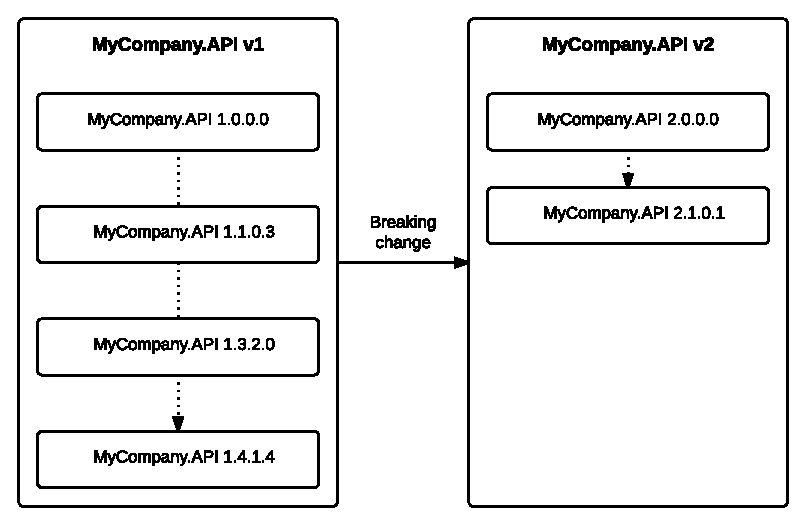
\includegraphics[width=8cm]{img/version-identifying.pdf}}
\caption{Incrementation of version identifiers}
\label{fig:version-identifying}
\end{figure} 


\subsection{Services version life-cycle}
Services version life-cycle defines the time period in which a version should be maintained. If the time is short, customers don't have enough time for their upgrades required in order to switch to the new version. On the other hand if the period is too long, too many versions of services have to be maintained. The suitable time span is a result of consideration of each individual organization with respect to their capability to deal with changes.

If there are too many versions maintained at the same time, there might be a requirement to lower the maintenance costs. In order to do so a mechanism is needed to identify and remove obsolete versions. One such mechanism is counting active services consumers. For example there are three clients each of them uses different version. Client 1 uses services v1, client 2 uses v2 and the last client uses v3. All version have to be maintained. After the client 1 switches from v1 to v3 the version v1 is no longer used and can be removed (figure \ref{fig:version-life-cycle}).

\begin{figure}[htp] \centering{
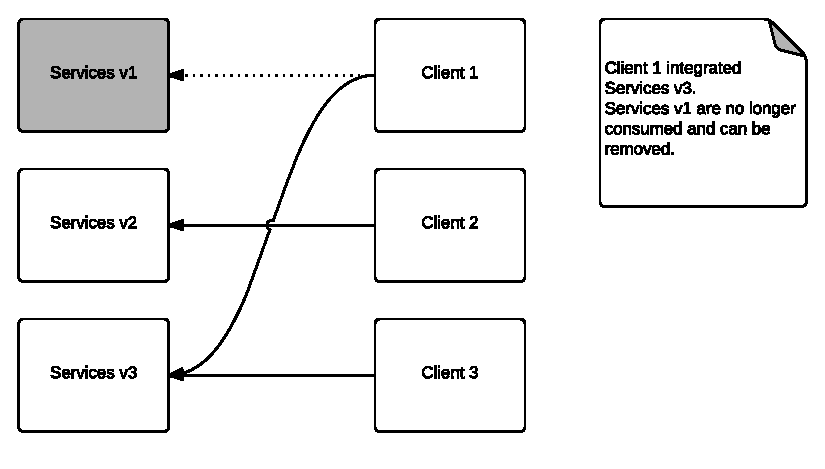
\includegraphics[width=10cm]{img/version-life-cycle.pdf}}
\caption{Version lifecycle}
\label{fig:version-life-cycle}
\end{figure} 



%This lifecycle is possible only when the service method versioning approach is implemented, in case of whole-service versioning, when the service is given into state deprecated, it is equivalent to its removal. New agreement between the provider and consumer is needed, so that consumer have to implement changes to use the new service. %or just keep using the older version. The whole-service versioning provides less flexibility.

\section{Services deployment}
The deployment goal is to deliver a high quality product to the consumer. Deployment management and their strategy has the responsibility to produce such a product. After the services are developed they should be well tested to prove their quality. If consumers requirements are fulfilled, the services are deployed to a production environment.

\subsection{Environments}
To get a good quality service API, it is quite necessary to have more environments running the same API version. Every environment has its role. There are at least two of them - development and production. Development environment is one with the latest version and is usually continuously developed. The production environment contains a stable version used by consumers.

In order to test the functionality of API it is inevitable to have more than two mentioned environments. There should be at least one environment dedicated to testing and one environment which runs a stable version. The last one is generally named as staging environment. It simulates the production environment to provide to producer a test environment where the API is running. It can discover application failures before the main release to the production environment happens. On figure \ref{fig:environments} is shown the possible composition of environments.

\begin{figure}[htp] \centering{
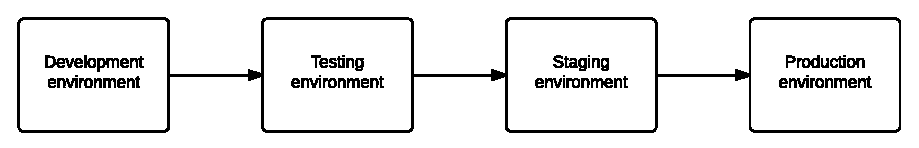
\includegraphics[width=10cm]{img/environments.pdf}}
\caption{Environments architecture}
\label{fig:environments}
\end{figure} 


On figure \ref{fig:consumer-server} is shown the case when one environment holds just one version of API. If another version is needed to be made available, it has to be deployed on another server. Then customers are using different servers. In fact, thanks to the service versioning, one environment can run more than one version of API. The environment usage is again dependent on specific deployment architecture.

\begin{figure}[htp] \centering{
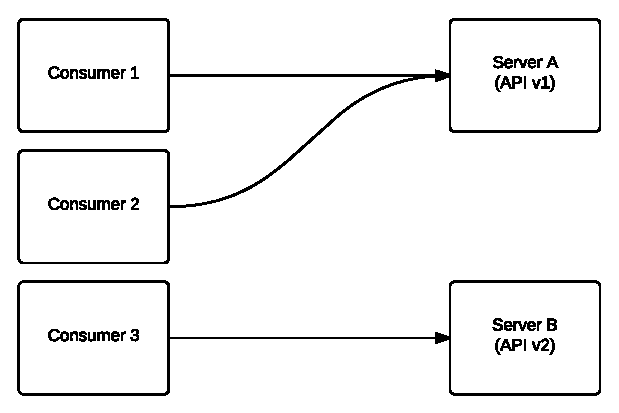
\includegraphics[width=8cm]{img/consumer-server.pdf}}
\caption{Possible usage of two deployed versions of API}
\label{fig:consumer-server}
\end{figure} 


\subsection{Deployment strategy}
One of the approaches how to release a new version of API is cutover, the other one is parallel development. The cutover requires downtime period planning. The downtime determines when a cutover occurs. 

The parallel deployment allows to have more versions on which the development, testing and consuming are proceeding (figure \ref{fig:parellel-development}). This approach offers more reliability, because of running backup system but requires more effort from provider and consumers (e.g. maintenance, customer testing). When a new version is going to be released, it is deployed to an environment but keeps the old system running on its environment continues with development, support and usage of the old one. 

\begin{figure}[htp] \centering{
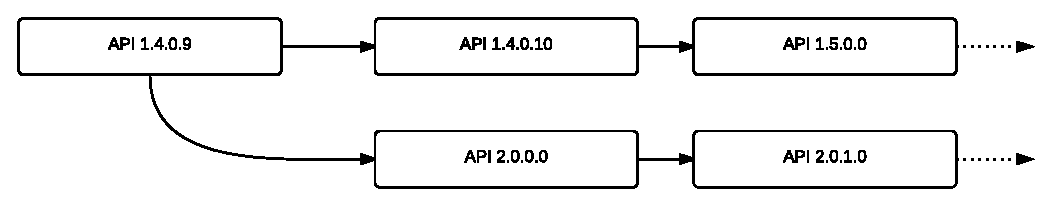
\includegraphics[width=10cm]{img/parellel-development.pdf}}
\caption{Parallel development}
\label{fig:parellel-development}
\end{figure} 

Having cutover approach when the actual version of API on the development environment is going to be emitted to the production, the developed code version number increases (figure \ref{fig:cutover-development}). Then development of a new version starts. The cut version is, after being stable, released to the production. 

\begin{figure}[htp] \centering{
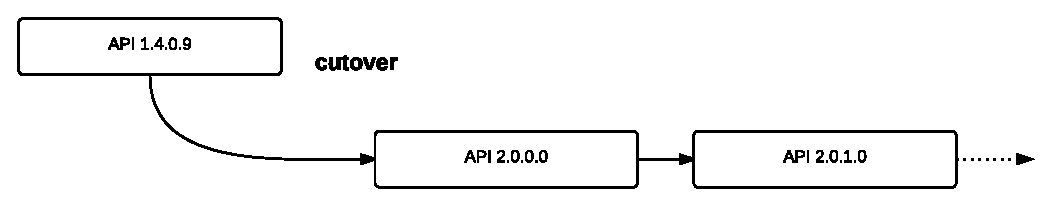
\includegraphics[width=10cm]{img/cutover-development.pdf}}
\caption{Cutover development}
\label{fig:cutover-development}
\end{figure}  


\subsection{Deployment methods}
There are more possibilities how to deploy the API to an environment. The whole API can be copied and deployed manually or it can be used a third party tool to manage deployments:

\begin{enumerate}
  \item{Manual method} \hfill \\
  The API image is copied to a new environment manually. This method is network based and provide diminution of distribution time and assistance in updates. On the other hand there can be problems with accessing the files on network and other with determining the reason of possible system fails. 
  \item{Continuous integration method} \hfill \\
  The \gls{scm} (SCM) to assist the distribution of the system. SCM server contains the master version of the API, developers work with its local version and after making some changes they push them to the server. Having the most recent version depends just on simple update from SCM server to get the last revision (what is revision was explained in Section \ref{subsec:versionid}). The SCM tool has a history of changes within a files. Developers can see every change done on the file from its creation to its newest version. When a change causes a failure of function of software, it can be reverted.
  
  With the SCM is connected a practice called Continuous Integration (CI). When someone push a change of a file to the SCM, the continuous integration ensures the build process and testing of whole project. The new change is integrated into the implemenation. If the CI build or tests fails it is possible to see which file caused the failure. 
  Result of the build process is a \gls{dll} file. This file is deployed to environments. The CI tool can partially or totally asist the deployment process. The process is shown on figure \ref{fig:deployment-process}.
  
\begin{figure}[htp] \centering{
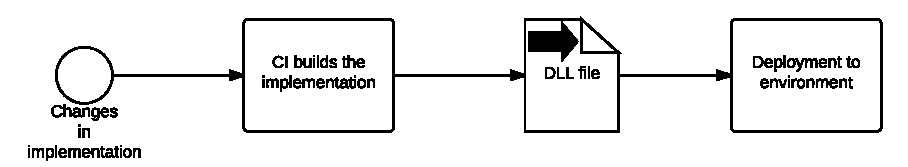
\includegraphics[width=11cm]{img/deployment-process.pdf}}
\caption{Contunuous Integration and DLL deployment}
\label{fig:deployment-process}
\end{figure} 
   
\end{enumerate}


\section{Versioning of services}
\label{sec:verioningservices}
There are three levels of interpretation of a \emph{service} as was already described in section \ref{subsec:levels-of-service}. A change and consequent creation of a new version can occur within each of this levels - service implementation, service interface and business abstraction.

\subsection{Versioning of service implementation}
The implementation of a service can be changed. The new version of service can be either backward compatible or backward incompatible. The implementation is encapsulated below the interface and is not visible for outer world. It can be modified without affecting clients. The backward compatible changes in this level can be a simple bug fix. The incompatible changes are modifications which influence the service calls responses.

Every change of the implementation leads to the versioning of the code but not necessarily to versioning of API. The version are identified by more than one digits which increase according to versioning strategy. For example, major digit increment by breaking changes, minor digit by compatible changes. Compatible changes can be done without a new version of API. In case of a breaking change, also API is versioned. 

\subsection{Versioning of service interface}
Service interface is an entry point for consumers to work with the services. Interface can be versioned as well and its change impacts the consumer application. Compatible change of the interface is an addition of an action. On the other side non compatible change is a removal of an action. When a new action is added, no one is using it and it is optional if somebody would make use of it. When an action is removed, consumers which are using it are negatively affected and their implementation can be broken.

\subsection{Versioning of business service}
Sometimes it is needed to change the business service. It means the business which is abstracted have to be changed. For example because of new requirements due to legislative a business service needs modifications. If this kind of change affects behaviour, semantic or functionality of existing service. In this case, it is easier to create a new service rather than a new version. 
